\documentclass{article}


\usepackage{PRIMEarxiv}

\usepackage[utf8]{inputenc} % allow utf-8 input
\usepackage[T1]{fontenc}    % use 8-bit T1 fonts
\usepackage{hyperref}       % hyperlinks
\usepackage{url}            % simple URL typesetting
\usepackage{booktabs}       % professional-quality tables
\usepackage{amsfonts}       % blackboard math symbols
\usepackage{nicefrac}       % compact symbols for 1/2, etc.
\usepackage{microtype}      % microtypography
\usepackage{siunitx}
\usepackage{hyperref}
\sisetup{per-mode=symbol}
\usepackage{lipsum}
\usepackage{parskip}
\usepackage{fancyhdr}       % header
\usepackage{graphicx}       % graphics
\graphicspath{{images/}}     % organize your images and other figures under media/ folder

%Header
\pagestyle{fancy}
\thispagestyle{empty}
\rhead{ \textit{ }} 

% Update your Headers here
\fancyhead[LO]{Aim Is All You Need}
% \fancyhead[RE]{Firstauthor and Secondauthor} % Firstauthor et al. if more than 2 - must use \documentclass[twoside]{article}



  
%% Title
\title{Aim Is All You Need}

\author{
  Seth Katz \\
  \texttt{\{katzseth22202@gmail.com} \\
}


\begin{document}
\maketitle

\begin{abstract}\label{sec:abstract}
 In 2017, Google Research published ``Attention is All You Need" \cite{vaswani2023attentionneed}.  Their paper introduced the Transformer, which let neural networks capture long range dependencies.   Just a few years later, OpenAI developed tools like ChatGPT \cite{chatgpt} that resemble hypothetical early prototypes of the computers in Star Trek \cite{startrek}.

But here's the bittersweet truth:  While our screens flicker with progress, the tangible realms of space, energy and paleontology remain comparatively stagnant.

\textbf{Dude, Where's my spaceeship?}

This paper's goal is to enable our progress in physical realms to catch up with our progress online.  Our journey requires applying a single unifying idea that is much simpler than attention - aim.   \begin{figure}[h]
    \centering
    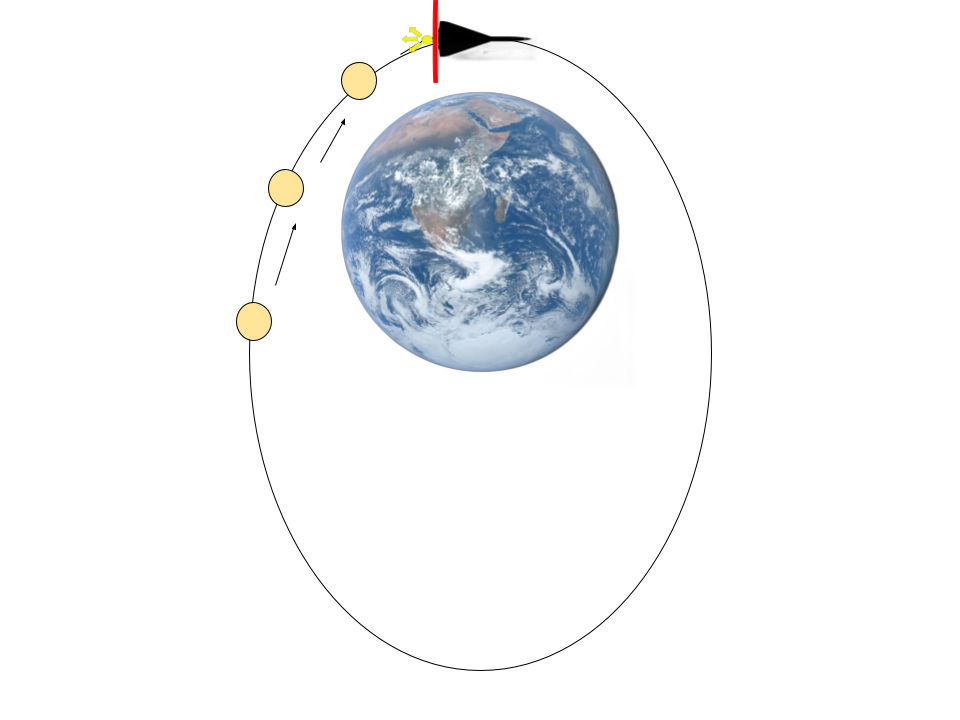
\includegraphics[width=0.5\linewidth]{images/Starship_Impact_ellipse.png}
    \caption{Balloons from a first rocket crash (not shown) crash into a second target rocket and provide propulsion}
    \label{fig:balloon_impact}
\end{figure}

Consider two rockets.   The first deploys a series of fast moving balloons capable of small navigation adjustments.  As shown in \autoref{fig:balloon_impact} these balloons precisely follow a path to crash  into a separate  target rocket.   These precise collisions deliver high-density jolts of pulsed energy and momentum to the target vehicle, enabling a surprisingly broad range of groundbreaking applications.    

Just as neural networks enabled consumer AI, they potentially allow us to achieve the precision control to make this externally pulsed propulsion concept feasible.

\textbf{A Checklist of Grand Challenges Externally Pulsed Propulsion Can Solve}
\begin{itemize}
    \item 
Suborbital Transit:  We'll create a viable suborbital travel vehicle allowing passengers to take off from normal airport runways and reach anywhere in the world in less than 2 hours.   Noise pollution near population centers will be no worse than it is with conventional aircraft.
 \item Rocket Revolution: We'll end the tyranny of the rocket equation.   We'll still use small rockets, but giant rockets with high propellant mass fraction will no longer be needed to reach orbit.   
 
 \item Lunar Lift-off: Launching from the moon may still require volatiles, but not the more difficult task of making and storing high performance rocket fuel.
  \item Jurassic Dark: As a side effect of our advances, we'll create the field of lunar paleontology and discover concrete evidence for how life originated on Earth.  We'll build a genetic record of extinct species from ancient geological periods, like the dinosaurs. 
  \item Straw Ways to Heaven:   We can construct terrestrial megastructures, extending from the ground to the edge of space, without relying on advanced magnetic technologies such as Lofstrom Launch Loops \cite{lofstrom_loop}. A particularly ambitious yet beneficial example might be a vacuum tube connecting Earth and space, a "Straw Way to Heaven."
  \item Carbon Cancelled: We will solve our energy problems with carbon negative fuel that absorbs the carbon dioxide produced by industry, all while using minimal land and resources
  \item Moon mining:  We'll develop in-situ resource utilization (ISRU) technology, first on our moon and then on icy moons like Saturn's moon Phoebe
\end{itemize}
Note, this paper summarizes some of the ideas in the blog ``Aim Is All You Need"\cite{aim2024}.
\end{abstract}

\section{Introduction}
Project Orion, conceived in the 1950s, remains the sole propulsion method based on mature contemporary technology that offers both high specific impulse and high thrust \cite{projorion}. Its mechanism involved propelling a spacecraft by directing hypervelocity plasma from nuclear explosions onto a pusher plate. Despite its theoretical promise, Orion faced insurmountable challenges related to political feasibility, radioactive fallout, and the impractical mass requirements stemming from the high minimum yield of nuclear explosions. Nevertheless, Orion conceptually validated the physics of hypervelocity pulsed propulsion.

Our approach replaces nuclear bombs with precisely aimed, hypervelocity gas balloons impacting a rocket's pusher plate. These balloons can be downscaled to practical sizes, and unlike nuclear explosions, small hypervelocity impacts could potentially be efficiently contained within a pulsed reaction chamber.

Leveraging gravity assists and the Oberth effect \cite{oberth_effect}, hypervelocity balloons could achieve energy densities and specific impulses comparable to Project Orion. This approach wouldn't demand nuclear or massive photovoltaic power, and it would enable lunar launches that use polar volatiles directly without needing to produce rocket fuel.     

Traditional control and localization techniques combined with recent neural network advancements raises the probability of achieving the extremely precise navigation for externally pulsed propulsion.

\section{To the moon by water balloon.  Getting to orbit with External Pulsed Propulsion}
\subsection{Making Starship's excess capacity useful to satellite customers}
SpaceX's Starship \cite{starship} rocket may be the first fully reusable rocket. At scale, this could dramatically reduce space flight costs.   However, the rocket's large payload size is probably too big for today's space industry needs. For example, in \textit{The New York Times}
\begin{quote}
Carissa Christensen, the chief executive of Bryce Tech, an analytics firm that tracks the launch market, says launching Starship frequently will be key to closing SpaceX’s business case, but finding customers to fill the rocket’s giant payload capacity will be challenging. 
"Starship's payload capacity is huge; it's very, very big, and there aren't that many commercial uses today for a rocket that big," she said.  "Maybe it'll be so cheap that it makes sense to launch satellites on it if its not full or near full."  \cite{nyt_starship_size}
\end{quote}
Although many satellites might be too small to fill up Starship, they can still be very expensive to build and test. For an extreme example, the James Webb Telescope \cite{james_webb_space_telescope} cost \9.7 billion dollars \cite{jwst_cost} to build. This McKinsey report argues 
\begin{quote}
Safety and reliability will continue to be overarching concerns, suggesting excellent execution will be table stakes for a competitive launch company. \cite{mckinsey_reliability}
\end{quote}
Once rockets start ferrying astronauts, reliability becomes even more emphatically nonnegotiable. What if there was a way to use Starship's huge size to make its valuable payloads less vulnerable to rapid unscheduled disassembly? 


%Bibliography
\bibliographystyle{unsrt}  
\bibliography{references}  


\end{document}
